% !TEX root=./adl.tex

\section{Optimizers: From Adam to Muon}

% -----------------------------------------------------------------------
\subsection{The Adam Optimizer}

% -----------------------------------------------------------------------
\begin{frame}{Adam: Adaptive Moment Estimation~\cite{kingma2015adam}}

  \begin{columns}[T]
    \begin{column}{0.50\textwidth}
      \textbf{Key idea:} Maintain per-parameter running estimates of gradient mean and variance, then scale updates adaptively.

      \vspace{0.3em}
      \begin{algorithm}[H]
        \small
        \caption{Adam}
        \KwInput{LR $\eta$, decay rates $\beta_1, \beta_2$, $\epsilon$}
        Initialize $\vm_0 = 0, \vv_0 = 0$\;
        \For{$t = 1, 2, \ldots$}{
          $\vg_t \gets \nabla_{\vw} L(\vw_{t-1})$\;
          $\vm_t \gets \beta_1 \vm_{t-1} + (1 - \beta_1) \vg_t$\;
          $\vv_t \gets \beta_2 \vv_{t-1} + (1 - \beta_2) \vg_t^2$\;
          $\hat{\vm}_t \gets \vm_t / (1 - \beta_1^t)$\;
          $\hat{\vv}_t \gets \vv_t / (1 - \beta_2^t)$\;
          $\vw_t \gets \vw_{t-1} - \eta \cdot \hat{\vm}_t / (\sqrt{\hat{\vv}_t} + \epsilon)$\;
        }
      \end{algorithm}
    \end{column}
    \begin{column}{0.47\textwidth}
      \textbf{Components:}
      \begin{description}[leftmargin=0.3em, labelwidth=\widthof{\bfseries Bias corr.}]
        \item[$\vm_t$] First moment (mean): momentum-smoothed gradient
        \item[$\vv_t$] Second moment (variance): tracks gradient magnitude per parameter
        \item[Bias corr.] $\hat{\vm}_t, \hat{\vv}_t$ correct the zero-initialization bias
        \item[$1/\sqrt{\hat{\vv}_t}$] Rescales each parameter's update inversely to its gradient magnitude
      \end{description}

      \vspace{0.3em}
      \textbf{Defaults:} $\beta_1 {=} 0.9$, $\beta_2 {=} 0.999$, $\epsilon {=} 10^{-8}$

      \vspace{0.3em}
      \textbf{LLM defaults:} $\beta_2 {=} 0.95$, weight decay via AdamW~\cite{loshchilov2019adamw}
    \end{column}
  \end{columns}
\end{frame}

% -----------------------------------------------------------------------
\begin{frame}{Adam's Per-Parameter Adaptivity}

  Adam normalizes each gradient coordinate independently:
  \[
    \Delta w_i \;\propto\; \frac{\hat{m}_i}{\sqrt{\hat{v}_i} + \epsilon}
    \qquad \Rightarrow \qquad |\Delta w_i| \approx \pm \eta
  \]

  \vspace{0.3em}
  \textbf{Advantages:}
  \begin{itemize}
    \item Parameters with sparse/small gradients still get meaningful updates
    \item Relatively insensitive to gradient scale $\Rightarrow$ less LR tuning
    \item Works well across different parameter types (embeddings, attention, MLP)
  \end{itemize}

  \vspace{0.3em}
  \textbf{Limitation for matrix parameters:}
  \begin{itemize}
    \item Adam treats each entry $W_{ij}$ independently
    \item Ignores the \emph{matrix structure} of weight updates
    \item The gradient $G = \nabla_W L$ often has high condition number: a few singular values dominate
    \item Adam's element-wise rescaling does not fix this directional imbalance
  \end{itemize}

  \vspace{0.3em}
  $\Rightarrow$ Can we design an optimizer that respects the matrix structure of 2D parameters?

\end{frame}

% -----------------------------------------------------------------------
\subsection{The Muon Optimizer}

% -----------------------------------------------------------------------
\begin{frame}{Muon: Momentum + Orthogonalization~\cite{jordan2024muon}}

  \textbf{Key insight:} For 2D weight matrices, \emph{orthogonalize} the momentum buffer before applying the update. This ensures all singular directions are updated equally.

  \vspace{0.4em}
  \begin{columns}[T]
    \begin{column}{0.50\textwidth}
      \textbf{Algorithm overview:}
      \begin{enumerate}
        \item Compute gradient $G_t = \nabla_W L$
        \item Accumulate with \textbf{Nesterov momentum}:
        \[
          M_t = \beta \cdot M_{t-1} + G_t
        \]
        \item \textbf{Orthogonalize} the momentum via Newton-Schulz iteration:
        \[
          U_t = \text{NS}_5(M_t) \approx \text{Ortho}(M_t)
        \]
        \item Update: $W_t = W_{t-1} - \eta \cdot U_t$
      \end{enumerate}

      \vspace{0.3em}
      {\small Apply Muon only to 2D (matrix) parameters.\\
      Use AdamW for embeddings, classifier head, biases, and all 1D parameters.}
    \end{column}
    \begin{column}{0.47\textwidth}
      \textbf{What does orthogonalization do?}

      Given $G = U \Sigma V^\top$ (SVD), the nearest semi-orthogonal matrix is:
      \[
        \text{Ortho}(G) = U V^\top
      \]

      This \emph{replaces all singular values with 1}:

      \vspace{0.2em}
      \begin{center}
      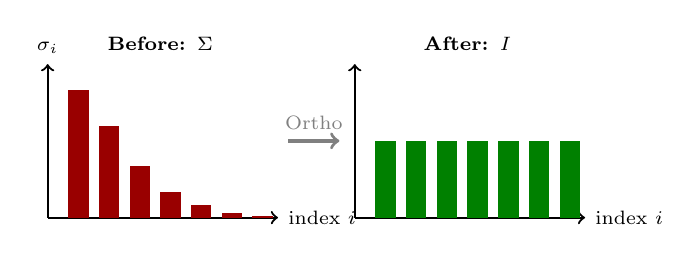
\begin{tikzpicture}[scale=0.65]
        % Before
        \draw[->, thick] (0,0) -- (4.5,0) node[right, font=\scriptsize] {index $i$};
        \draw[->, thick] (0,0) -- (0,3) node[above, font=\scriptsize] {$\sigma_i$};
        \node[font=\scriptsize\bfseries] at (2.2,3.4) {Before: $\Sigma$};
        \foreach \i/\h in {0.4/2.5, 1.0/1.8, 1.6/1.0, 2.2/0.5, 2.8/0.25, 3.4/0.1, 4.0/0.03} {
          \fill[red!60!black] (\i,0) rectangle (\i+0.4, \h);
        }
        % After
        \begin{scope}[shift={(6,0)}]
          \draw[->, thick] (0,0) -- (4.5,0) node[right, font=\scriptsize] {index $i$};
          \draw[->, thick] (0,0) -- (0,3) node[above, font=\scriptsize] {};
          \node[font=\scriptsize\bfseries] at (2.2,3.4) {After: $I$};
          \foreach \i in {0.4, 1.0, 1.6, 2.2, 2.8, 3.4, 4.0} {
            \fill[green!50!black] (\i,0) rectangle (\i+0.4, 1.5);
          }
        \end{scope}
        \draw[->, very thick, gray] (4.7, 1.5) -- (5.7, 1.5) node[midway, above, font=\scriptsize] {Ortho};
      \end{tikzpicture}
      \end{center}

      {\scriptsize Rare gradient directions (small $\sigma_i$) get amplified to the same scale as dominant ones.}
    \end{column}
  \end{columns}
\end{frame}

% -----------------------------------------------------------------------
\begin{frame}{Why Orthogonalize? The Condition Number Problem}

  \begin{columns}[T]
    \begin{column}{0.52\textwidth}
      \textbf{Observation:} Gradient matrices for 2D transformer parameters typically have \emph{very high condition numbers}.

      \vspace{0.3em}
      A few singular directions dominate the update, while most directions receive negligible signal.

      \vspace{0.3em}
      \textbf{SGD/Adam behavior:}
      \begin{itemize}
        \item SGD: all neuron updates dominated by the top few singular vectors
        \item Adam: element-wise rescaling partially helps, but does not fix the directional imbalance
      \end{itemize}

      \vspace{0.3em}
      \textbf{Orthogonalization:}
      \begin{itemize}
        \item Sets all singular values to 1
        \item Every direction in the update gets equal weight
        \item ``Amplifies rare directions'' that have small magnitude but are important for learning
      \end{itemize}
    \end{column}
    \begin{column}{0.45\textwidth}
      \begin{center}
        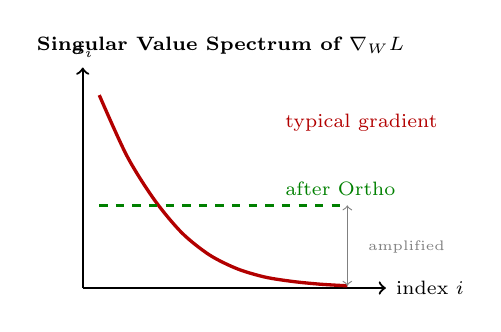
\begin{tikzpicture}[scale=0.7]
          % Singular value spectrum
          \draw[->, thick] (0,0) -- (5.5,0) node[right, font=\scriptsize] {index $i$};
          \draw[->, thick] (0,0) -- (0,4) node[above, font=\scriptsize] {$\sigma_i$};
          \node[font=\scriptsize\bfseries] at (2.5,4.4) {Singular Value Spectrum of $\nabla_W L$};

          % Typical gradient spectrum - steep decay
          \draw[red!70!black, very thick, smooth] plot coordinates {
            (0.3, 3.5) (0.8, 2.4) (1.3, 1.6) (1.8, 1.0) (2.3, 0.6)
            (2.8, 0.35) (3.3, 0.2) (3.8, 0.12) (4.3, 0.07) (4.8, 0.04)
          };
          \node[font=\scriptsize, red!70!black, anchor=west] at (3.5, 3.0) {typical gradient};

          % After orthogonalization - flat
          \draw[green!50!black, very thick, dashed] (0.3, 1.5) -- (4.8, 1.5);
          \node[font=\scriptsize, green!50!black, anchor=west] at (3.5, 1.8) {after Ortho};

          % Annotation
          \draw[<->, gray, thin] (4.8, 0.04) -- (4.8, 1.5);
          \node[font=\tiny, gray, anchor=west] at (5.0, 0.75) {amplified};
        \end{tikzpicture}
      \end{center}

      \vspace{0.3em}
      \textbf{Connection to steepest descent:}

      Orthogonalized gradient $UV^\top$ is the \emph{steepest descent direction} under the \textbf{spectral norm}~\cite{bernstein2024oldoptimizer}:
      \[
        UV^\top = \arg\min_{\|D\|_\text{op} \leq 1} \langle G, D \rangle
      \]
    \end{column}
  \end{columns}
\end{frame}

% -----------------------------------------------------------------------
\subsection{Newton-Schulz Iteration}

% -----------------------------------------------------------------------
\begin{frame}{Newton-Schulz Iteration for Fast Orthogonalization}

  Computing SVD is expensive ($O(nm^2)$ for $n \times m$). The \textbf{Newton-Schulz (NS) iteration} approximates orthogonalization using only matrix multiplications.

  \vspace{0.3em}
  \textbf{One NS step} for matrix $X$ with SVD $X = U S V^\top$:
  \[
    X' = a X + b (X X^\top) X + c (X X^\top)^2 X
  \]
  In terms of singular values, this applies a quintic polynomial:
  \[
    \phi(s) = a \cdot s + b \cdot s^3 + c \cdot s^5
  \]

  After $N$ steps: $X_N = U\, \phi^{(N)}(S)\, V^\top$, where $\phi^{(N)}$ is the $N$-fold composition.

  \vspace{0.3em}
  \textbf{Goal:} Choose $a, b, c$ so that $\phi^{(N)}(s) \to 1$ for all $s \in (0, 1]$ as fast as possible.

  \vspace{0.3em}
  \textbf{Requirements:}
  \begin{itemize}
    \item $\phi(1) = 1$ (fixed point): $a + b + c = 1$
    \item $\phi'(1) = 0$ (stable fixed point): $a + 3b + 5c = 0$
    \item $\phi(s) \to 1$ quickly for $s$ near $0$ (fast convergence for small singular values)
  \end{itemize}

\end{frame}

% -----------------------------------------------------------------------
\begin{frame}{Tuning Newton-Schulz Coefficients}

  \begin{columns}[T]
    \begin{column}{0.50\textwidth}
      \textbf{Baseline coefficients} (standard in literature):
      \[
        (a, b, c) = (2,\; -1.5,\; 0.5)
      \]
      Slow convergence near $s = 0$: many iterations needed.

      \vspace{0.4em}
      \textbf{Optimized coefficients}~\cite{jordan2024muon}:
      \[
        (a, b, c) = (3.4445,\; -4.7750,\; 2.0315)
      \]
      Much steeper growth near $s = 0$ $\Rightarrow$ \textbf{only 5 iterations suffice} for good approximation.

      \vspace{0.4em}
      \textbf{Implementation detail:}
      \begin{itemize}
        \item Normalize $X \gets X / \|X\|_F$ so singular values lie in $[0, 1]$
        \item Runs entirely in \textbf{bfloat16}
        \item If matrix is tall ($n > m$), transpose before iterating
      \end{itemize}
    \end{column}
    \begin{column}{0.47\textwidth}
      \textbf{Single NS polynomial $\phi(s)$:}
      \begin{center}
        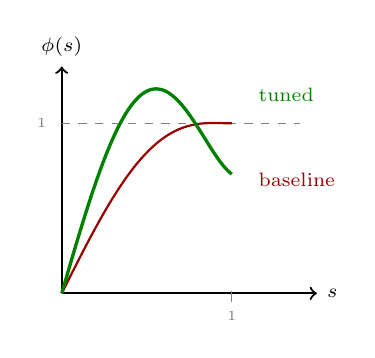
\begin{tikzpicture}[scale=0.72]
          \draw[->, thick] (0,0) -- (4.5,0) node[right, font=\scriptsize] {$s$};
          \draw[->, thick] (0,0) -- (0,4) node[above, font=\scriptsize] {$\phi(s)$};
          % y=1 reference
          \draw[gray, dashed, thin] (0,3) -- (4.2,3);
          \node[font=\tiny, gray, anchor=east] at (-0.1,3) {$1$};
          % Tick at s=1
          \draw[gray, thin] (3,0.05) -- (3,-0.15);
          \node[font=\tiny, gray, below] at (3,-0.15) {$1$};

          % Baseline: phi(s) = 2s - 1.5s^3 + 0.5s^5, scaled: x axis 0..3 maps to s 0..1, y axis *3
          \draw[red!60!black, thick, domain=0:3, samples=80, smooth]
            plot (\x, {3*(2*(\x/3) - 1.5*(\x/3)^3 + 0.5*(\x/3)^5)});
          \node[font=\scriptsize, red!60!black, anchor=west] at (3.3, 2.0) {baseline};

          % Tuned: phi(s) = 3.4445s - 4.775s^3 + 2.0315s^5, scaled
          \draw[green!50!black, very thick, domain=0:3, samples=80, smooth]
            plot (\x, {3*(3.4445*(\x/3) - 4.775*(\x/3)^3 + 2.0315*(\x/3)^5)});
          \node[font=\scriptsize, green!50!black, anchor=west] at (3.3, 3.5) {tuned};
        \end{tikzpicture}
      \end{center}

      \textbf{After 5 iterations $\phi^{(5)}(s)$:}
      \begin{center}
        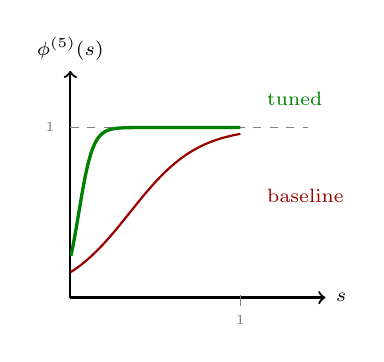
\begin{tikzpicture}[scale=0.72]
          \draw[->, thick] (0,0) -- (4.5,0) node[right, font=\scriptsize] {$s$};
          \draw[->, thick] (0,0) -- (0,4) node[above, font=\scriptsize] {$\phi^{(5)}(s)$};
          \draw[gray, dashed, thin] (0,3) -- (4.2,3);
          \node[font=\tiny, gray, anchor=east] at (-0.1,3) {$1$};
          \draw[gray, thin] (3,0.05) -- (3,-0.15);
          \node[font=\tiny, gray, below] at (3,-0.15) {$1$};

          % Baseline after 5 iters: slow convergence, still curved
          \draw[red!60!black, thick, domain=0.01:3, samples=80, smooth]
            plot (\x, {3*min(1, max(0, 0.5 + 0.5*tanh(2.5*(\x/3 - 0.35))))});
          \node[font=\scriptsize, red!60!black, anchor=west] at (3.3, 1.8) {baseline};

          % Tuned after 5 iters: nearly step function
          \draw[green!50!black, very thick, domain=0.01:3, samples=80, smooth]
            plot (\x, {3*min(1, max(0, 0.5 + 0.5*tanh(min(5, max(-5, 12*(\x/3 - 0.05))))))});
          \node[font=\scriptsize, green!50!black, anchor=west] at (3.3, 3.5) {tuned};
        \end{tikzpicture}
      \end{center}
      {\scriptsize Tuned coefficients converge to a near-step function after 5 iterations: $\phi^{(5)}(s) \approx 1$ for all $s > 0$.}
    \end{column}
  \end{columns}
\end{frame}

% -----------------------------------------------------------------------
\begin{frame}[fragile]{Newton-Schulz Implementation}

  The complete NS orthogonalization in PyTorch:

  \vspace{0.3em}
  \begin{center}
  \begin{minipage}{0.85\textwidth}
    \begin{tcolorbox}[colback=slide_blue!15, colframe=slide_blue!70, boxrule=0.5pt, arc=3pt, left=4pt, right=4pt, top=3pt, bottom=3pt]
    {\small
\begin{verbatim}
def newtonschulz5(G, steps=5, eps=1e-7):
    a, b, c = (3.4445, -4.7750, 2.0315)
    X = G.bfloat16()
    X /= (X.norm() + eps)  # normalize to [0,1]
    if G.size(0) > G.size(1):
        X = X.T              # work on smaller dim
    for _ in range(steps):
        A = X @ X.T
        B = b * A + c * A @ A
        X = a * X + B @ X   # quintic polynomial
    if G.size(0) > G.size(1):
        X = X.T
    return X
\end{verbatim}
    }
    \end{tcolorbox}
  \end{minipage}
  \end{center}

  \vspace{0.3em}
  \textbf{Computational cost per NS step} (for $n \times m$ matrix, $m \leq n$):
  \begin{itemize}
    \item $XX^\top$: $2nm^2$ FLOPs, then $A \cdot A$: $2m^3$ FLOPs, then $B \cdot X$: $2nm^2$ FLOPs
    \item Total per step: $\leq 6nm^2$ FLOPs. \quad For 5 steps: $30nm^2$ FLOPs
    \item \textbf{Relative overhead:} $\leq 5m/B$ of the forward pass (where $B$ = batch size in tokens)
    \item Negligible for typical LLM training batch sizes ($B \gg m$)
  \end{itemize}

\end{frame}

% -----------------------------------------------------------------------
\begin{frame}{Full Muon Algorithm}

  \begin{columns}[T]
    \begin{column}{0.52\textwidth}
      \begin{algorithm}[H]
        \small
        \caption{Muon Optimizer}
        \KwInput{LR $\eta$, momentum $\beta$, NS steps $T{=}5$}
        Initialize $M_0 = 0$ for each 2D param $W$\;
        \For{$t = 1, 2, \ldots$}{
          $G_t \gets \nabla_W L(\vw_{t-1})$\;
          \tcp{Nesterov momentum}
          $M_t \gets \beta \cdot M_{t-1} + G_t$\;
          $\tilde{M}_t \gets \beta \cdot M_t + G_t$\;
          \tcp{Orthogonalize via NS}
          $U_t \gets \text{NewtonSchulz}_T(\tilde{M}_t)$\;
          \tcp{Update weights}
          $W_t \gets W_{t-1} - \eta \cdot U_t$\;
        }
      \end{algorithm}

      \vspace{0.3em}
      \textbf{Practical details:}
      \begin{itemize}
        \item Muon: 2D weight matrices (Q, K, V, MLP)
        \item AdamW: embeddings, output head, biases, LayerNorm
        \item Apply to Q, K, V \emph{separately}, not concatenated
      \end{itemize}
    \end{column}
    \begin{column}{0.45\textwidth}
      \begin{center}
        \begin{tikzpicture}[
          box/.style={draw, rounded corners=3pt, minimum width=2.8cm, minimum height=0.6cm, font=\small, align=center, inner sep=3pt},
          arr/.style={->, thick, >=stealth},
          scale=0.85
        ]
          \node[box, fill=slide_beige!50] (grad) at (0, 0) {Gradient $G_t$};
          \node[box, fill=slide_blue!50] (mom) at (0, -1.5) {Nesterov\\Momentum $\tilde{M}_t$};
          \node[box, fill=slide_green!70] (ns) at (0, -3.0) {Newton-Schulz\\$\text{NS}_5(\tilde{M}_t)$};
          \node[box, fill=green!30] (ortho) at (0, -4.5) {Orthogonal\\Update $U_t$};
          \node[box, fill=gray!15] (update) at (0, -6.0) {$W_t = W_{t-1} - \eta U_t$};

          \draw[arr] (grad) -- (mom);
          \draw[arr] (mom) -- (ns);
          \draw[arr] (ns) -- (ortho);
          \draw[arr] (ortho) -- (update);

          % Side annotations
          \node[font=\tiny, gray, anchor=west, align=left] at (1.8, -1.5) {smooths gradient\\over time};
          \node[font=\tiny, gray, anchor=west, align=left] at (1.8, -3.0) {5 mat-muls\\in bfloat16};
          \node[font=\tiny, gray, anchor=west, align=left] at (1.8, -4.5) {all $\sigma_i = 1$};
        \end{tikzpicture}
      \end{center}
    \end{column}
  \end{columns}
\end{frame}

% -----------------------------------------------------------------------
\begin{frame}{Connection to Shampoo}

  \textbf{Shampoo}~\cite{gupta2018shampoo} is a second-order optimizer that preconditions gradients using accumulated outer products.

  \vspace{0.3em}
  \textbf{Instantaneous Shampoo update} (without accumulation):
  \[
    W_{t+1} = W_t - \eta \cdot (G_t G_t^\top)^{-1/4}\, G_t\, (G_t^\top G_t)^{-1/4}
  \]

  Substituting SVD $G_t = U \Sigma V^\top$:
  \begin{align*}
    (G G^\top)^{-1/4} &= (U \Sigma^2 U^\top)^{-1/4} = U \Sigma^{-1/2} U^\top \\
    (G^\top G)^{-1/4} &= (V \Sigma^2 V^\top)^{-1/4} = V \Sigma^{-1/2} V^\top
  \end{align*}

  Therefore:
  \[
    (G G^\top)^{-1/4}\, G\, (G^\top G)^{-1/4}
    = U \Sigma^{-1/2} \cdot \Sigma \cdot \Sigma^{-1/2} V^\top
    = U V^\top
  \]

  \begin{alertblock}{Key equivalence}
    Muon (without momentum) $=$ instantaneous Shampoo.\\
    Both reduce to the orthogonalized gradient $UV^\top$.\\
    Muon replaces Shampoo's expensive preconditioner accumulation with a lightweight NS iteration.
  \end{alertblock}

\end{frame}

% -----------------------------------------------------------------------
\begin{frame}{Muon Results}

  \begin{columns}[T]
    \begin{column}{0.50\textwidth}
      \textbf{NanoGPT speedrunning benchmark:}
      \begin{itemize}
        \item Muon achieves \textbf{1.35$\times$ faster training} to target validation loss on FineWeb
        \item After introduction (Oct 2024), Muon was used in \textbf{all 12 subsequent records} set by 7 different researchers
        \item Muon has slower per-step wallclock time than AdamW (due to NS overhead) $\Rightarrow$ its persistent adoption is strong evidence of genuine sample-efficiency gains
      \end{itemize}

      \vspace{0.3em}
      \textbf{1.5B parameter scale:}
      \begin{itemize}
        \item GPT-2 XL-level HellaSwag in \textbf{10 8xH100-hours} vs.\ 13.3 hours for AdamW
      \end{itemize}

      \vspace{0.3em}
      \textbf{CIFAR-10:}
      \begin{itemize}
        \item Speed record: 3.3 $\to$ 2.6 A100-seconds for 94\% accuracy
      \end{itemize}
    \end{column}
    \begin{column}{0.47\textwidth}
      \begin{center}
        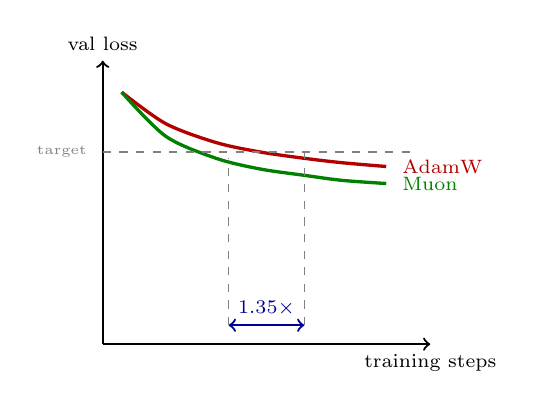
\begin{tikzpicture}[scale=0.8]
          \draw[->, thick] (0,0) -- (5.2,0) node[below, font=\scriptsize] {training steps};
          \draw[->, thick] (0,0) -- (0,4.5) node[above, font=\scriptsize] {val loss};

          % Adam curve - slower
          \draw[red!70!black, very thick, smooth] plot coordinates {
            (0.3, 4.0) (1.0, 3.5) (1.8, 3.2) (2.5, 3.05) (3.2, 2.95)
            (3.8, 2.88) (4.5, 2.82)
          };
          \node[font=\scriptsize, red!70!black, anchor=west] at (4.6, 2.82) {AdamW};

          % Muon curve - faster
          \draw[green!50!black, very thick, smooth] plot coordinates {
            (0.3, 4.0) (1.0, 3.3) (1.8, 2.95) (2.5, 2.78) (3.2, 2.68)
            (3.8, 2.60) (4.5, 2.55)
          };
          \node[font=\scriptsize, green!50!black, anchor=west] at (4.6, 2.55) {Muon};

          % Target line
          \draw[gray, dashed] (0, 3.05) -- (5, 3.05);
          \node[font=\tiny, gray, anchor=east] at (-0.1, 3.05) {target};

          % Speedup annotation
          \draw[<->, thick, blue!60!black] (2.0, 0.3) -- (3.2, 0.3);
          \node[font=\scriptsize, blue!60!black, above] at (2.6, 0.3) {1.35$\times$};
          \draw[gray, thin, dashed] (2.0, 0.3) -- (2.0, 2.95);
          \draw[gray, thin, dashed] (3.2, 0.3) -- (3.2, 3.05);
        \end{tikzpicture}
      \end{center}
      {\scriptsize Schematic of Muon vs AdamW training curves. Muon reaches the same validation loss with fewer steps.}

      \vspace{0.3em}
      \textbf{Why trust these results?}

      The NanoGPT speedrunning task is a \emph{competitive benchmark}: researchers are incentivized to find the best optimizer. If Muon were worse, competitors would discard it. Its persistent adoption across records by independent researchers is strong evidence.
    \end{column}
  \end{columns}
\end{frame}

% -----------------------------------------------------------------------
\begin{frame}{Muon: Summary and Practical Advice}

  \begin{block}{Key Takeaways}
    \begin{itemize}
      \item \textbf{Muon = Momentum + Orthogonalization} via Newton-Schulz iteration
      \item Orthogonalization ensures all singular directions get equal-magnitude updates
      \item Equivalent to steepest descent under the spectral norm
      \item Mathematically equivalent to instantaneous (accumulation-free) Shampoo
      \item Newton-Schulz iteration: 5 steps of matrix multiplications in bfloat16, negligible overhead
      \item 1.35$\times$ sample-efficiency improvement over AdamW on NanoGPT benchmark
    \end{itemize}
  \end{block}

  \vspace{0.3em}
  \textbf{When to use:}
  \begin{description}[leftmargin=0.3em, labelwidth=\widthof{\bfseries Muon + AdamW}]
    \item[Muon] All 2D weight matrices: Q, K, V projections, MLP layers (apply separately, not concatenated)
    \item[AdamW] Embeddings, output head, biases, LayerNorm/RMSNorm parameters, all 1D tensors
  \end{description}

  \vspace{0.3em}
  \textbf{Prior work:} Orthogonal-SGDM~\cite{tuddenham2022orthogonal}, Stochastic Spectral Descent~\cite{carlson2015stochastic}
\end{frame}
